\chapter{Theory and Concepts of Intelligent Clinical Document Processing with SNOMED CT Coding}

Natural language processing and intelligent document understanding have become increasingly important in modern healthcare systems due to the growing volume of unstructured clinical information generated through Electronic Health Records and related medical documentation. Effective extraction and interpretation of meaningful information from clinical narratives require an understanding of several underlying concepts and technologies that form the foundation of intelligent healthcare solutions. Key areas such as natural language processing principles, transformer-based architectures, clinical ontologies, and document understanding techniques collectively enable automated analysis of healthcare documents. Mathematical models and learning mechanisms further support these approaches by providing the theoretical basis for training, optimization, and prediction tasks within the proposed system. The concepts presented in this chapter establish the theoretical foundation necessary for understanding the design and implementation of the Intelligent Clinical Document Processing System (ICDPS).

\section{Introduction to Natural Language Processing and AI in Healthcare}
Natural Language Processing (NLP) is a subfield of artificial intelligence (AI) concerned with enabling computers to understand, interpret, and generate human language. NLP encompasses a broad range of tasks including tokenization, part-of-speech tagging, syntactic parsing, semantic analysis, information extraction, machine translation, and text generation.

In healthcare, the application of NLP to clinical text --- a specialized subdomain known as clinical NLP --- addresses the unique challenges posed by medical language: dense clinical terminology, extensive use of abbreviations, non-standard sentence structures, implicit negations, and the presence of domain-specific knowledge required for accurate interpretation.

Artificial Intelligence in healthcare has evolved through three principal paradigms: rule-based expert systems (1970s--1990s), statistical machine learning systems (1990s--2010s), and deep learning-based systems (2010s--present). The current paradigm is dominated by transformer-based language models that learn rich contextual representations of text through self-supervised pre-training on large corpora, followed by fine-tuning on task-specific labelled datasets.

\section{Fundamental Concepts of Natural Language Processing}
Natural Language Processing (NLP) provides the computational techniques required for transforming unstructured textual information into meaningful representations that can be processed and interpreted by machine learning systems. Clinical text presents additional challenges compared to general language because of its specialized terminology, abbreviations, domain-specific expressions, and variations in writing styles across healthcare environments. Effective processing of clinical narratives requires several fundamental operations that enable systems to understand contextual meaning and identify medically relevant information. Concepts such as text preprocessing, entity extraction, and contextual interpretation mechanisms form the foundation of intelligent clinical document understanding systems. These concepts collectively support accurate information extraction and facilitate downstream tasks such as summarization, classification, and standardized clinical coding.
\subsection{Text Preprocessing}
Text preprocessing transforms raw clinical text into a normalized form suitable for model input. Key preprocessing steps include:

\begin{description}
    \item[Sentence Boundary Detection:] Identifying sentence boundaries in clinical text is non-trivial due to the presence of medical abbreviations (e.g., ``b.d.'' for twice daily) that contain internal periods. Rule-based boundary detectors are commonly supplemented with statistical models trained on clinical corpora.
    \item[Tokenization:] Clinical text tokenizers must handle compound medical terms, hyphenated expressions, and numeric values with units. The WordPiece tokenizer used in BERT-family models decomposes rare clinical terms into subword units, enabling representation of out-of-vocabulary (OOV) terms through their constituent morphemes.
    \item[Normalization:] Clinical text normalization includes case normalization, expansion of abbreviations using a clinical abbreviation lexicon, and standardization of numeric expressions (e.g., dates, dosages). Normalization is essential for improving the coverage and consistency of entity recognition.
    \item[Stop Word Removal:] While stop word removal is common in document classification tasks, it is generally avoided in clinical named entity recognition (NER) because short function words may carry clinical significance (e.g., ``no'' indicating negation, ``in'' indicating anatomical location).
\end{description}

\subsection{Named Entity Recognition}
Named Entity Recognition (NER) is the task of identifying spans of text that refer to entities of predefined types. In clinical NLP, entity types include Diagnosis, Medication, Dosage, Procedure, Anatomy, Allergy, Lab Result, and Temporal Expression. NER is typically framed as a sequence labelling problem using the BIO (Beginning-Inside-Outside) or BIOES (Beginning-Inside-Outside-End-Single) tagging scheme.

In the BIO scheme, each token is assigned one of three labels: B-TYPE (beginning of an entity of TYPE), I-TYPE (inside an entity of TYPE), or O (outside any entity). For example, the phrase ``type 2 diabetes mellitus'' would be tagged as:
\begin{align*}
\text{``type''} &\rightarrow \text{B-DIAGNOSIS} \\
\text{``2''} &\rightarrow \text{I-DIAGNOSIS} \\
\text{``diabetes''} &\rightarrow \text{I-DIAGNOSIS} \\
\text{``mellitus''} &\rightarrow \text{I-DIAGNOSIS}
\end{align*}

Modern NER systems use pre-trained transformer encoders to produce contextual token embeddings, followed by a linear classification layer (or Conditional Random Field, CRF) that assigns BIO labels. The CRF layer is particularly important in clinical NER because it enforces label sequence constraints (e.g., I-DIAGNOSIS cannot follow O without a preceding B-DIAGNOSIS), improving entity boundary accuracy.

\subsection{Negation and Uncertainty Detection}
Clinical text frequently contains negated or uncertain assertions that must be correctly identified to avoid coding non-existent conditions. The statement ``no evidence of pneumonia'' should not result in a SNOMED CT code for pneumonia. Negation detection algorithms identify trigger phrases (e.g., ``no'', ``absent'', ``denies'', ``without'') and apply a scoping rule to mark nearby clinical entities as negated.

The NegEx algorithm \cite{ref14} uses a set of manually defined trigger phrase lists and applies a fixed-window scope rule. More recent approaches employ neural models that learn negation scope from annotated corpora, achieving higher recall on complex negation patterns including long-distance and nested negations.

\section{Transformer Architecture and BERT-Based Models}
The evolution of deep learning in Natural Language Processing has led to the development of transformer-based architectures that overcome several limitations of traditional recurrent and sequential models. Earlier approaches such as Recurrent Neural Networks (RNNs) and Long Short-Term Memory (LSTM) networks process text sequentially, making it difficult to efficiently capture long-range dependencies and increasing computational complexity for large textual datasets. The transformer architecture introduced an attention-based mechanism that enables parallel processing of sequences while preserving contextual relationships between words. This architecture has become the foundation for modern language models such as BERT, BioBERT, ClinicalBERT, and other domain-specific transformer variants used in healthcare applications. The general architecture of a transformer model, consisting of encoder-decoder blocks, multi-head self-attention mechanisms, positional encoding, and feed-forward networks, is illustrated in Fig. \ref{fig:transformer_architecture}. This architecture provides the underlying framework for contextual representation learning and forms the basis for the language models used in the proposed Intelligent Clinical Document Processing System (ICDPS).

\subsection{The Transformer Architecture}
The transformer architecture, introduced by Vaswani et al. \cite{ref76} in 2017, replaced recurrent neural networks with a fully attention-based design. The key innovation is the multi-head self-attention mechanism, which allows each position in the input sequence to attend to all other positions simultaneously, enabling the model to capture long-range dependencies without the sequential bottleneck of RNNs.

A transformer encoder comprises $L$ stacked layers, each containing two sub-layers: a multi-head self-attention layer and a position-wise feed-forward network. Layer normalization and residual connections are applied around each sub-layer. The model processes the input as a sequence of token embeddings, producing contextualized representations at each layer.

The self-attention mechanism computes attention weights as:
\begin{equation}
\text{Attention}(Q, K, V) = \text{softmax}\left(\frac{QK^T}{\sqrt{d_k}}\right) V
\label{eq:self_attention}
\end{equation}
where $Q$, $K$, and $V$ are the query, key, and value matrices derived from the input embeddings, and $d_k$ is the dimension of the key vectors. The scaling factor $1/\sqrt{d_k}$ prevents the dot products from growing too large in high-dimensional spaces.

\begin{figure}[htbp]
\centering
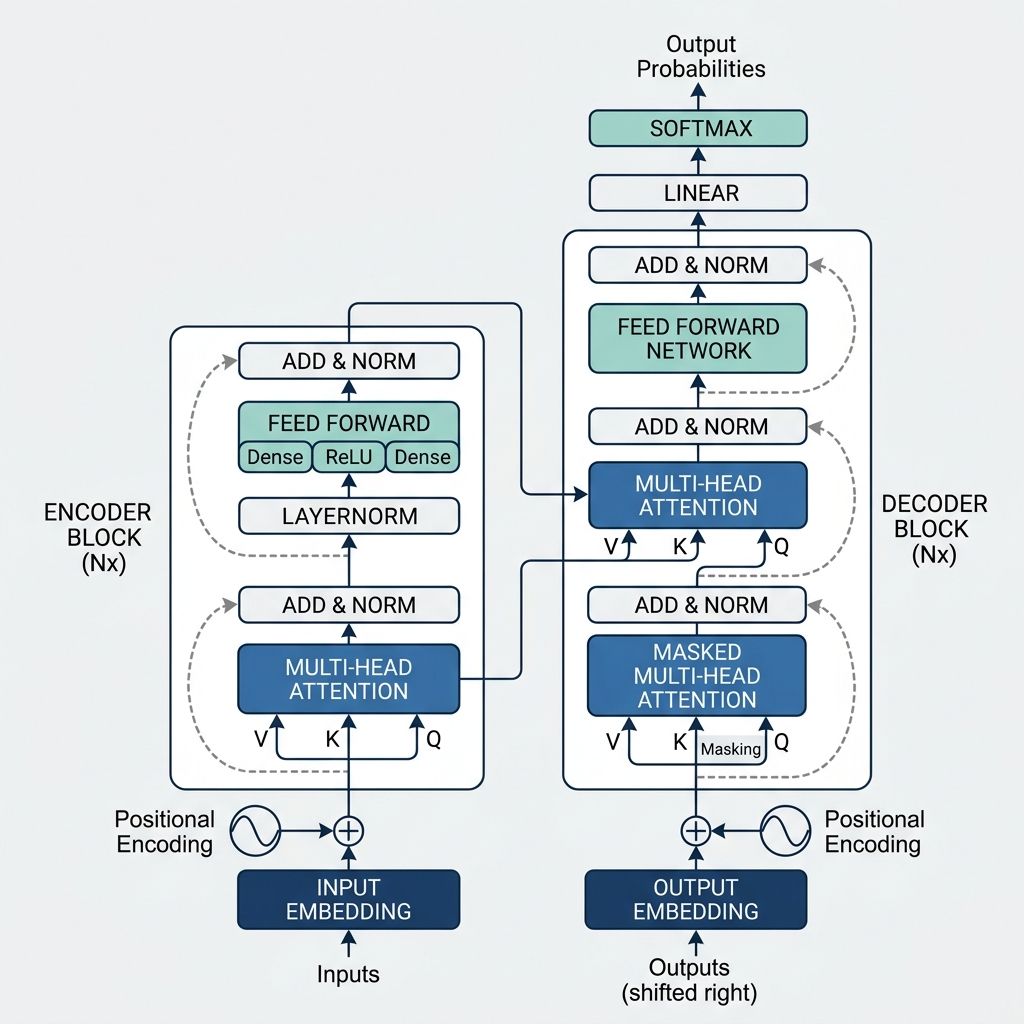
\includegraphics[width=0.8\textwidth]{Figures/transformer_architecture}
\caption{Transformer model architecture}
\label{fig:transformer_architecture}
\end{figure}

\subsection{BERT Pre-Training and Fine-Tuning}
BERT (Bidirectional Encoder Representations from Transformers) \cite{ref8} is a transformer encoder pre-trained on two self-supervised tasks: Masked Language Modelling (MLM) and Next Sentence Prediction (NSP). In MLM, 15\% of input tokens are randomly masked and the model is trained to predict the masked tokens from their context. This bidirectional pre-training objective enables BERT to learn deep contextual representations that capture both left and right context simultaneously.

Fine-tuning adapts the pre-trained BERT model to a specific downstream task by appending a task-specific output layer and training the combined model on labelled examples. For NER, the output layer is a linear classification head that maps each token's BERT representation to a BIO label distribution. Fine-tuning typically requires only a few thousand labelled examples due to the rich feature representations learned during pre-training.

\subsection{BioBERT for Biomedical NLP}
BioBERT \cite{ref1} initializes from the BERT-base weights and continues pre-training on approximately 4.5 billion words from PubMed abstracts and 13.5 billion words from PMC full-text articles. This domain-adaptive pre-training exposes the model to biomedical terminology, clinical abbreviations, and domain-specific syntactic patterns, resulting in significantly improved performance on biomedical NER, relation extraction, and question answering tasks compared to BERT trained exclusively on general-domain text.

For clinical NER tasks using the i2b2 datasets, BioBERT achieves $F_1$-scores of 0.886 on the 2010 dataset and 0.895 on the 2012 dataset, outperforming previous state-of-the-art systems by 2--4 percentage points.

\section{SNOMED CT: Structure and Coding Principles}
SNOMED CT (Systematized Nomenclature of Medicine --- Clinical Terms) is one of the most comprehensive and widely adopted clinical terminology systems used for representing medical concepts in a standardized manner. It provides a structured framework for organizing clinical knowledge and enables semantic interoperability across healthcare systems. By using standardized codes and concept relationships, SNOMED CT facilitates consistent representation of diagnoses, procedures, findings, medications, and other clinical entities. In the proposed Intelligent Clinical Document Processing System (ICDPS), SNOMED CT plays a critical role in transforming extracted clinical information into standardized representations that can support efficient storage, retrieval, and interoperability. The following sections discuss the ontology structure of SNOMED CT and the principles involved in the coding process. 

\subsection{Ontology Structure}
SNOMED CT is a formally structured clinical terminology comprising three primary components: Concepts, Descriptions, and Relationships. A Concept is a unique clinical idea identified by a numeric concept identifier (\texttt{conceptId}). Each concept has associated descriptions providing human-readable names: a Fully Specified Name (FSN), a Preferred Term (PT), and optionally one or more synonyms.

Relationships between concepts encode semantic associations. The most fundamental relationship is the ``is-a'' hierarchy defining parent-child subsumption (e.g., ``Type 2 diabetes mellitus'' is-a ``Diabetes mellitus''). Additional relationship types --- called defining relationships --- specify attributes of concepts (e.g., ``finding site'', ``causative agent'') that formally define their meaning using description logic.

SNOMED CT is organized into hierarchies including Clinical Finding, Procedure, Observable Entity, Body Structure, Organism, Substance, Pharmaceutical/Biologic Product, and Qualifier Value. These hierarchies correspond to the entity categories recognized by the ICDPS extraction engine.

\subsection{SNOMED CT Coding Process}
Clinical coding with SNOMED CT requires selecting the most specific concept that accurately represents the clinical entity described in the source document. This process involves:
\begin{enumerate}
    \item[(i)] identifying the target entity type (finding, procedure, substance, etc.);
    \item[(ii)] retrieving candidate concepts from the SNOMED CT release; and
    \item[(iii)] selecting the concept whose FSN and synonyms best match the clinical context.
\end{enumerate}

Automated SNOMED CT coding systems must contend with several challenges: synonym variability (multiple clinical terms may map to the same concept), compositional expressions (clinical descriptions may combine multiple SNOMED CT concepts), and contextual sensitivity (the appropriate code may depend on information outside the entity mention itself, such as negation status, laterality, or severity).

\section{Document Understanding and OCR}
Clinical documents are often available in diverse formats such as scanned reports, PDFs, image-based records, and structured templates, requiring efficient methods for extracting machine-readable information. Document understanding combines computer vision and natural language processing techniques to identify document structure, reading order, and semantic content. Optical Character Recognition (OCR) forms an essential component of this process by converting textual information embedded in images into digital text suitable for downstream processing. Additionally, semantic retrieval mechanisms such as vector similarity search improve the identification and mapping of extracted concepts. The following subsections discuss OCR techniques and vector-based retrieval methods used in the proposed system.

\subsection{Optical Character Recognition}
Optical Character Recognition (OCR) converts images of printed or handwritten text into machine-readable character sequences. Modern OCR engines such as Tesseract 5.0 \cite{ref36} use LSTM-based sequence models trained on large character recognition datasets. The OCR pipeline comprises image preprocessing (binarization, deskewing, noise removal), layout analysis (identifying text regions, columns, and reading order), and character recognition (generating character sequences from text regions).

OCR performance on clinical documents varies significantly with document quality. Printed clinical letters typically achieve character error rates below 2\%, while aged or low-quality scans may exhibit higher error rates. Post-OCR error correction using clinical dictionaries improves text quality for downstream NLP tasks.

\subsection{Vector Similarity Search}
Vector similarity search is used in the SNOMED CT candidate retrieval module to find concepts whose text descriptions are semantically similar to the extracted clinical entity. Each SNOMED CT concept description is represented as a dense vector using FastText embeddings \cite{ref17}, and an approximate nearest-neighbour search using FAISS (Facebook AI Similarity Search) retrieves the top-$K$ most similar candidates based on cosine similarity.

FAISS provides efficient indexing and retrieval for high-dimensional vector collections using quantization and graph-based algorithms. For the SNOMED CT index containing approximately 1.5 million concept descriptions, FAISS enables sub-second retrieval with approximate search accuracy exceeding 98\% relative to exact search.

\section{Mathematical Foundations}
The implementation of transformer-based language models and clinical entity extraction systems relies on several mathematical concepts that govern model learning and performance evaluation. Mathematical formulations provide the basis for converting model outputs into probability distributions, optimizing learning processes, and assessing predictive performance. Concepts such as loss functions, optimization strategies, and evaluation metrics are essential for understanding how the proposed system learns meaningful representations from clinical text and measures its effectiveness. The following subsections discuss the mathematical principles employed in the proposed framework. 

\subsection{Softmax and Cross-Entropy Loss}
The NER classification head applies the softmax function to convert raw logit scores into a probability distribution over BIO labels:
\begin{equation}
P(y = k \mid x) = \frac{\exp(z_k)}{\sum_{j} \exp(z_j)}
\label{eq:softmax}
\end{equation}
where $z_k$ is the logit for class $k$. The model is trained to minimize the cross-entropy loss:
\begin{equation}
\mathcal{L} = -\sum_{i=1}^{N} \log P(y = y_i \mid x_i)
\label{eq:cross_entropy}
\end{equation}
where $y_i$ is the true label for token $i$. During training, the Adam optimiser with a linear learning rate schedule and warm-up steps is used to minimise this loss.

\subsection{Evaluation Metrics}
NER performance is evaluated using token-level precision ($P$), recall ($R$), and F1-score ($F1$):
\begin{equation}
P = \frac{\text{TP}}{\text{TP} + \text{FP}}
\label{eq:precision}
\end{equation}
\begin{equation}
R = \frac{\text{TP}}{\text{TP} + \text{FN}}
\label{eq:recall}
\end{equation}
\begin{equation}
F1 = \frac{2 \cdot P \cdot R}{P + R}
\label{eq:f1_score}
\end{equation}
where TP is the number of correctly predicted entity tokens, FP the number of incorrectly predicted entity tokens, and FN the number of entity tokens missed by the model. SNOMED CT mapping performance is evaluated using $\text{Precision}@K$, which measures the proportion of test instances where the correct SNOMED CT code appears in the top-$K$ suggestions.

\section{Comparison of Techniques}
Various approaches have been proposed for clinical information extraction and natural language processing tasks, ranging from traditional rule-based systems to modern transformer-based architectures. Each technique exhibits distinct characteristics in terms of training requirements, generalization capability, computational complexity, and overall performance. A comparative analysis of these techniques helps in understanding their strengths and limitations and provides a rationale for selecting an appropriate methodology for the proposed system. Table \ref{tab:ner_techniques_comparison} presents a comparison of commonly used approaches, including rule-based systems (e.g., cTAKES \cite{ref6}), BiLSTM-CRF models, and transformer-based methods across multiple evaluation criteria.

\begin{table}[htbp]
\centering
\caption{Comparison of Clinical NER Techniques}
\label{tab:ner_techniques_comparison}

\begin{tabular}{|p{3cm}|p{3.65cm}|p{3.75cm}|p{3.8cm}|}
\hline

\textbf{Criterion} &
\shortstack{\textbf{Rule-Based}\\\textbf{(cTAKES)}} &
\textbf{BiLSTM-CRF} &
\shortstack{\textbf{Transformer}\\\textbf{(BioBERT)}} \\

\hline

Training Data Required &
None (rules only) &
Moderate (annotated) &
Large (pre-training) + small (fine-tuning) \\

\hline

Generalization &
Low (template-dependent) &
Moderate &
High \\

\hline

Domain Adaptation &
Manual rule updates &
Re-training required &
Fine-tuning on small dataset \\

\hline

Clinical NER $F1$ &
0.72--0.78 &
0.80--0.85 &
0.88--0.93 \\

\hline

OOV Handling &
Poor &
Moderate (char features) &
Good (subword tokenization) \\

\hline

Inference Speed &
Fast &
Moderate &
Slower (GPU recommended) \\

\hline
\end{tabular}

\end{table}

\section*{Summary}
This chapter presented the theoretical foundations of the ICDPS, covering NLP fundamentals, the transformer architecture, BERT-based biomedical pre-training, SNOMED CT ontology structure, OCR technology, vector similarity search, and the mathematical principles underlying model training and evaluation. The comparative analysis demonstrated the superiority of transformer-based approaches over rule-based and BiLSTM-CRF methods for clinical NER tasks. Chapter 3 presents the detailed software requirements specification for the proposed system.
